\chapter{Sensor Modeling and Classification Methods
\label{chap:4}}

For this work, polyimide dielectric based capacitive load cells were chosen as the primary sensing apparatus
due to their prescribed robustness, low manufacture cost, and low power requirements.
Motivated by the selection of thin film polyimide, 
models for thin film deformation were studied for this work.
The deformation of polyimide is linear for thick films
and small deformations, but for thin films, 
on the mesoscale of dozens of micrometers,
polyimide films have nonlinear deformation.
These characteristics are manifested as creep, hysteresis, 
and temperature dependence.

To avoid problems in modeling caused by these reactions,
different approaches are used to determine rock material type and tool wear conditions 
from the sensor measurements. In the case presented in Ch.~\ref{chap:P3}, the sensor
film thickness has been dialed-in, and the measurements are much more linear with respect
to the input force. The sensor model for the linear sensor case is discussed in the next subsection,
after that, the classification methods used to avoid problems with creep, hysteresis, and temperature dependence
are discussed.

\subsection{Linear Sensor Modeling}

It is axiomatic that a linear and time-invariant sensor is an ideal sensor for measuring physical quantities.
Such a sensor would present an easily measured value that is a fixed multiple of another 
physical quantity that is desired to be measured without any dependence on the measurement history.
Such a sensor is difficult to attain, but non-ideal characteristics can still be modeled. 
Thin film deformation can be modeled using viscous elements, as shown in \ref{fig:sense_model}.
This is only an approximation, and depending on how nonlinear the dielectric deformation response is,
this model might not accurately capture the dynamics of the system.
The system overall is nonlinear, and with a material this viscous,
cycling the film rapidly will result in changes to the vibrational modes.

The stackup for the sensor membrane for the first iteration of the capacitive load cell
is shown in \ref{fig:stackupsense}. This model had a very thin inner layer, which resulted
in nonlinear dynamics. The next iteration of the sensor used a thicker membrane,
which resulted in a more linear sensor. 
The non-linearity of the first design was not an issue for tool wear or material classification,
but did impede using the measurements for force measurements. 

When considering the design of the more linear sensor, the model can be simplified to the 
linear case without a great loss in accuracy. The use of a small feed-forward neural network
are able to model the non-linearity present in the more linear design and further improve the accuracy.
The fact that a linear model is able to be used with the sensor and provide good accuracy means the sensor
is approaching ideal behavior.
The fact that a neural network model improves performance reveals that the system still has latent non-linearities.

Increasing the dielectric thickness will make it deform more linearly.
Increasing stiffness from the steel walls, $K_{walls}$, would also increase the sensor linearity.
Other types of capacitive sensor designs, like those which translate the electrodes overlapping areas,
are inherently more linear that the compressing plate design used for this research. However, for small
deformations, the hyperbolic relationship between capacitance and plate distance is approximately linear.

% Spring figure 
\begin{figure}[t]
    \centering
    \begin{circuitikz}
    \coordinate (A) at (-3.5, 0);
    \coordinate (B) at (-3.5, -2);
    \coordinate (C) at (0, 0);
    \coordinate (D) at (0, -2);
    \draw (A) to[spring] (B) ; 
    \node [right=4pt] at (-3.5, -1) {$K_{walls}$} ; % wall 1 spring
%    \draw (C) to[spring] (D) ; 
%    \node [right=4pt] at (3.0, -1) {$K_{w2}$} ; % wall 2 spring
    \draw (-1.80,-1.85) rectangle (1.8,-0.15);
    \draw (-1,-0.15) to[spring] (-1,-1.85) ;
    \draw (-0.15,-0.15) to[spring] (-0.15,-1.05) ;
    \draw (-0.15, -1.85) to[damper] (-0.15,-1.05) ;
    \node [right=8pt] at (0.15, -0.85) {\huge$\dots$};
    \node [right=4pt] at (1.00, -1.55) {$K_{p}$} ;  % polyimide spring
    \draw (0,0) to[short] (0, -0.15);
    \draw (0,-1.85) to[short] (0, -2);
    \draw (A) to[short] (C) ; % top bar
    \draw (B) to[short] (D) ; % bottom bar
    \draw (-1.2,-2) to[spring] (-1.2,-4) ; % bottom spring
    \node [right=4pt] at (-1.1, -3) {$K_{bottom}$} ;
    \draw (-1.2,0) to[spring] (-1.2,2) ; % top spring
    \node [right=4pt] at (-1.1, 1) {$K_{top}$} ;
    \draw [line width=0.5mm] (-3.2,-4) to (0.8,-4);
    \foreach \i in {-2,...,6} {
      \draw [line width=0.25mm] (\i/5 * 2- 2.1,-4) to (\i/5 * 2 - 1.6, -4.45);
    }
    \draw [line width=0.5mm] (-3.2,2) to (0.8,2);
    \draw [->] (-3,2) -- (-3,1.5) node [left] {$f(t)$};
    \end{circuitikz}
    \caption{A model of the sensor as a system of springs and dampers. 
             The PI can be modeled with a general visco-elastic model with
             repeating Maxwell elements. Here, it is summarized as $K_p$. 
             The springs representing the steel case top and bottom, $K_{top}$ and
             $K_{bottom}$, are much stiffer than the midsection. 
             Similarly, $K_{walls}$, of the steel case, is much stiffer than $K_p$.
             Thus the total device stiffness is readily approximated by 
             the stiffness of the device walls.}
    \label{fig:sense_model}
\end{figure}

% Stackup fig
\begin{figure}[]
\centering
\begin{tikzpicture}
    \node[anchor=south west, inner sep=0] (image) at (0,0) 
      {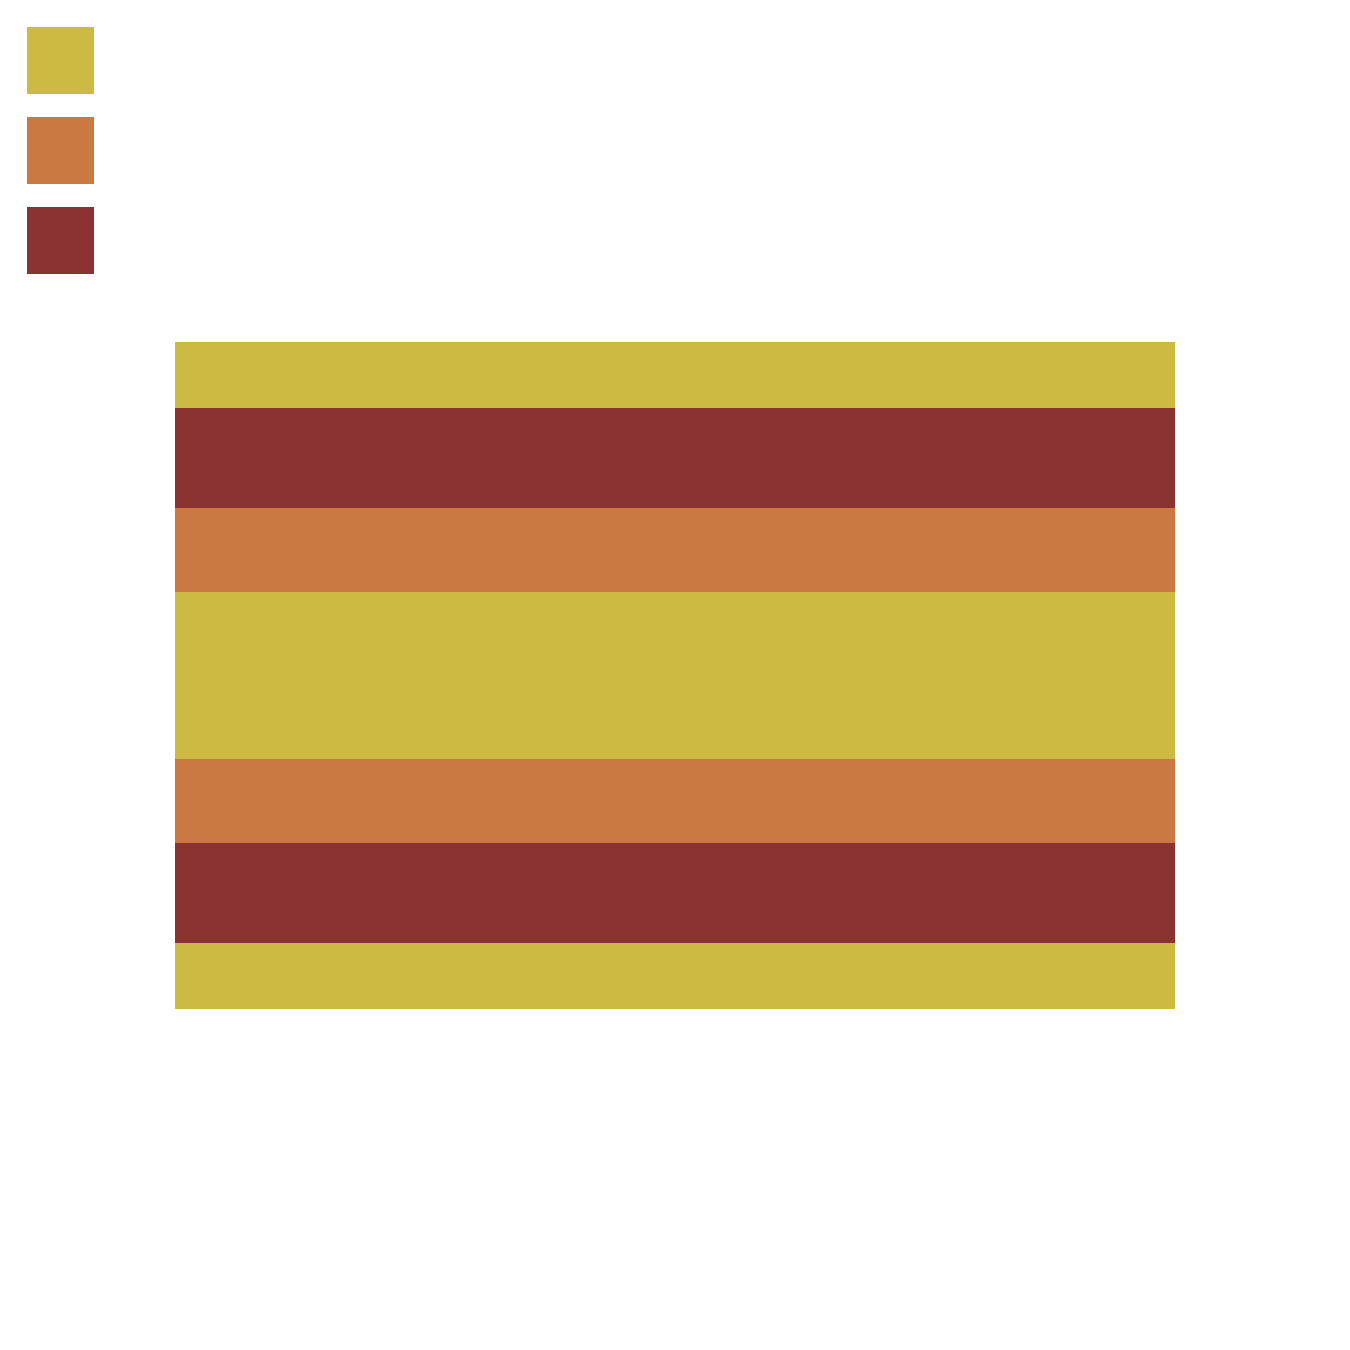
\includegraphics[trim=0 75 0 0,clip,width=0.55\linewidth]{figures/sensestackupxcf.png}};
    \begin{scope}[x={(image.south east)}, y={(image.north west)}]
      \node[anchor=west] at (0.08, 0.93) {Polyimide};
      \node[anchor=west] at (0.08, 0.845) {Copper};
      \node[anchor=west] at (0.08, 0.76) {Adhesive};
      \dimline {(0, 0.02)} {(0, 0.67)} {$100\mu$m};
%      \dimline {(1, 0.2)} {(1, 0.4)} {$d100\mu$m};
      \dimline[extension start length=-.50, extension end length=-.50]
                           {(.95, .28)} {(.95, .43)} {\small $25\mu$m};
      \dimline[extension start length=-1.500, extension end length=-1.500]
                           {(1, .43)} {(1, .51)} {\small $12\mu$m};
      \dimline[extension start length=-1.500, extension end length=-1.500]
                           {(.95, .61)} {(.95, .67)} {\small $12.5\mu$m};
      \dimline[extension start length=-1.500, extension end length=-1.500]
                           {(1, .10)} {(1, .18)} {\small $15\mu$m};
    \end{scope}
\end{tikzpicture}
\caption{The stackup for the FlexPCB sensing membrane. The outer PI layers are 12.5 $\mu$m
tall while the inner layer is 25 $\mu$m. The adhesive layers are 15 $\mu$m and the copper
layers are 12 $\mu$m. The total membrane height is about 100 $\mu$m. Due to the very thin
thickness of the dielectric film, the deformation characteristics will be dominated
by the interaction of the complex molecular chains and are expected to be nonlinear.
}
\label{fig:stackupsense}
\end{figure}

\subsection{Classification Methods}

Other items which govern the vibrational forces during cutting include
the material type and the tool wear. 
Different rock types have different fracture mechanics, 
and these differences can be measured and classified.
Different tool wear levels require different amounts of cutting force,
and will result in changing fracture mechanics dependent of the tool's geometry.

All of these changes in vibrational modes and forces can be tracked in the
frequency domain as changes to the emitted spectra. For this research,
it is known that energy is moving from certain vibrational
modes to other vibrational modes across the categories of material type
and tool wear. This shift in energy over the spectra can be measured
by using the magnitude of the Fourier transform coefficients for a 
short duration sample.

As the Fourier spectra magnitude coefficients change, these changes 
can be used to classify the conditions that caused them.
Data-driven classification techniques are used to identify these differences and 
predict the cutting conditions.
The methods are the K-Nearest Neighbors, the support-vector machine, and multilayer perceptron classifier.
These methods are able to categorize the different modal excitations present during different rock material and tool wear
conditions without needing the force measurement. 

For example, worn tools change the rock fracture process
to more of a crushing operation, resulting in lower and rumblier vibrations. 
Likewise, different materials will fracture in different patterns and frequencies due to their constitution.
On average, the statistical distribution of a measurement recorded 
during consistent rock material type and tool wear conditions
will differ from the distribution of a measurement recorded during different conditions.
This difference is identified by the classification methods and used to make classifications.

